\documentclass[12pt]{article}

\usepackage[top=5em, bottom=5em, left=5em, right=5em]{geometry}
\usepackage{listings}
\usepackage{tikz}
\usetikzlibrary{positioning}

\setlength\parindent{0em}
\setlength\parskip{1em}

\title {Assignment 4}

\author {Constantin Blach s4329872}

\begin{document}
\maketitle

This was done in collaboration with Hendrik Werner (s4549775).

\section{} %1
\section{} %2
\section{} %3
Dijkstra's algorithm produces wrong output for some graphs with negatively weighted edges such as this one:

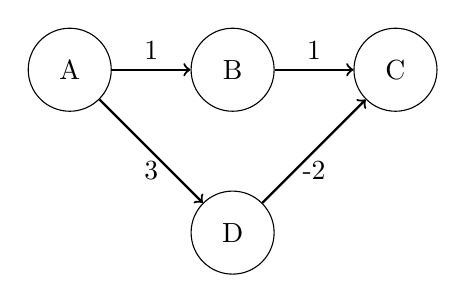
\begin{tikzpicture}[c/.style={circle, draw, minimum width=3em}]
	\node[c] (A) {A};
	\node[c, right=of A] (B) {B};
	\node[c, right=of B] (C) {C};
	\node[c, below=of B] (D) {D};

	\path[->, thick] (A) edge node[above] {1} (B);
	\path[->, thick] (A) edge node[below] {3} (D);
	\path[->, thick] (B) edge node[above] {1} (C);
	\path[->, thick] (D) edge node[below] {-2} (C);
\end{tikzpicture}

\section{} %4
I a max-heap the smallest element may reside inside a leaf node. This can be proven by a property of the heap: "If node $A$ is a parent of node $B$ then the value of $A$ is ordered with respect to the value of node B with the same ordering applying across the whole heap.". For a max-heap this ordering is $A > B$.

\begin{enumerate}
	\item \label{q4:a_is_smallest}
	We look at any non-leaf node $A$ and assume it contains the smallest element in the heap.
	\item \label{q4:b_is_smaller}
	According to our heap property child $B$ of node $A$ contains a smaller value than $A$.
	\item
	(\ref{q4:b_is_smaller}) and (\ref{q4:a_is_smallest}) contradict each other.
\end{enumerate}

By assuming that any non-leaf node contains the smallest element we get a contradiction the smallest value may only reside inside a leaf node.

\section{} %5
\section{} %6
Making all edge's weights non-negative by adding a constant to all edges is a valid method. This makes distances monotonically increasing. Dijksta's algorithm is greedy and always explores the node with the lowest distance.

We have out invariants:
\begin{itemize}
	\item $dist(A)$ is the shortest path from start $S$ to $A$ for each visited node $A$.
	\item $dist(X)$ is the shortest path from $S$ to $X$ we know of, for each unvisited node $X$.
\end{itemize}

With just one visited node they are obviously true.

We also assume this for $k$ visited nodes and choose the unvisited node $X$ for which $dist(X)$ is minimal (greedy) and $dist(X) = dist(A) + weight((A, X))$. $dist(X)$ must be minimal as if there were a shorter path to $X$ via another unvisited node $Y$ then $dist(Y)$ would need to be less than $dist(X)$ because the distance is monotonically increasing. This cannot be true according to our invariants because if $dist(Y) < dist(X)$ then $Y$ is explored before $X$.

\end{document}
